\documentclass{beamer}
\usepackage[outputdir=build]{minted}
\usepackage[skins,minted,breakable]{tcolorbox}
\usepackage[spanish]{babel}
\usepackage{subcaption}
\usetikzlibrary{matrix,backgrounds}
\usepackage{multirow}
\usepackage{multicol}
\graphicspath{ {../img/} {../../LaTeX/img/} {/home/csp98/latex/img/}}
\selectlanguage{spanish}
\usepackage[utf8]{inputenc}
\usetheme{PaloAlto}
\setbeamerfont{section in sidebar}{size=\fontsize{2}{4}\selectfont}
\setbeamerfont{subsection in sidebar}{size=\fontsize{2}{3}\selectfont}
\setbeamerfont{subsubsection in sidebar}{size=\fontsize{2}{2}\selectfont}

\setbeamerfont{section in toc}{size=\footnotesize}
\setbeamerfont{subsection in toc}{size=\scriptsize}
\setbeamerfont{subsubsection in toc}{size=\tiny}




\title{Práctica 2}
\date{6 de abril de 2018}
\subtitle{El elemento en su posición}

\author{María Jesús López Salmerón \\ Nazaret Román Guerrero \\ Laura Hernández Muñoz \\ José Baena Cobos  \\ Carlos Sánchez Páez}

\makeatletter
  \setbeamertemplate{sidebar \beamer@sidebarside}%{sidebar theme}
  {
    \beamer@tempdim=\beamer@sidebarwidth%
    \advance\beamer@tempdim by -6pt%
    \insertverticalnavigation{\beamer@sidebarwidth}%
    \vfill
    \ifx\beamer@sidebarside\beamer@lefttext%
    \else%
      \usebeamercolor{normal text}%
      \llap{\usebeamertemplate***{navigation symbols}\hskip0.1cm}%
      \vskip2pt%
    \fi%
}%
\makeatother

\subject{Algorítmica}
\AtBeginSection[]
  {
     \begin{frame}<beamer>
     \frametitle{Índice}
     \tableofcontents[currentsection]
     \end{frame}
  }
\AtBeginSubsection[]
{
  \begin{frame}<beamer>{Índice}
    \tableofcontents[currentsection,currentsubsection]
  \end{frame}
}

% Let's get started
\begin{document}
\centering
\begin{frame}
  \titlepage
\end{frame}

\begin{frame}{Índice}
  \tableofcontents
  % You might wish to add the option [pausesections]
\end{frame}

\section{Presentación del problema}

\begin{frame}[fragile]{El elemento en su posición}
Sea $v$ un vector \textbf{ordenado} y sin elementos repetidos, determinar si $\exists i : v[i]=i $
\end{frame}

\begin{frame}[fragile]{Ejemplos}
\begin{tikzpicture}[font=\ttfamily,
array/.style={matrix of nodes,nodes={draw, minimum size=7mm, fill=blue!30},column sep=-\pgflinewidth, row sep=0.5mm, nodes in empty cells,
row 1/.style={nodes={draw=none, fill=none, minimum size=5mm}}}]

\matrix[array] (array) {
0 & 1 & 2 & \textcolor{green}{3} & 4 & 5 & 6 & 7 & 8 & 9\\
  &   &   &   &   &   &   &   &   &   \\};
%\node[draw, fill=gray, minimum size=4mm] at (array-2-3) (box) {};
\node at (array-2-1) {-70};
\node at (array-2-2) {-35};
\node at (array-2-3) {0};
\node[draw, fill=green!20] at (array-2-4) {3};
\node at (array-2-5) {15};
\node at (array-2-6) {25};
\node at (array-2-7) {51};
\node at (array-2-8) {68};
\node at (array-2-9) {75};
\node at (array-2-10) {83};


\draw[<->]([yshift=-3mm]array-2-1.south west) -- node[below] {Tamaño del vector: 10} ([yshift=-3mm]array-2-10.south east);

\end{tikzpicture}
\vskip 0.5 cm
Resultado del algoritmo : \textbf{3}
\vskip 0.5 cm
\begin{tikzpicture}[font=\ttfamily,
array/.style={matrix of nodes,nodes={draw, minimum size=7mm, fill=blue!30},column sep=-\pgflinewidth, row sep=0.5mm, nodes in empty cells,
row 1/.style={nodes={draw=none, fill=none, minimum size=5mm}}}]

\matrix[array] (array) {
0 & 1 & 2 & 3 & 4 & 5 & 6 & 7 & 8 & 9\\
  &   &   &   &   &   &   &   &   &   \\};
%\node[draw, fill=gray, minimum size=4mm] at (array-2-3) (box) {};
\node at (array-2-1) {-70};
\node at (array-2-2) {-35};
\node at (array-2-3) {-2};
\node at (array-2-4) {1};
\node at (array-2-5) {15};
\node at (array-2-6) {25};
\node at (array-2-7) {51};
\node at (array-2-8) {68};
\node at (array-2-9) {75};
\node at (array-2-10) {83};

\draw[<->]([yshift=-3mm]array-2-1.south west) -- node[below] {Tamaño del vector: 10} ([yshift=-3mm]array-2-10.south east);

\end{tikzpicture}

\vskip 0.5 cm
Resultado del algoritmo : \textcolor{red}{\textbf{-1}}

\end{frame}

\section{Diseño de algoritmos}

\subsection{Algoritmo clásico}

\begin{frame}[fragile]{Clásico}
\begin{minted}[fontsize=\small]{c++}
  int elementoEnSuPosicion(const vector<int> &v) {
  	for (int i = 0; i < v.size() ; i++)
  		if (v[i] == i)
			return i;
	return -1;
  }
\end{minted}  
\end{frame}

\begin{frame}[fragile]{Ejemplo}
\begin{tikzpicture}[font=\ttfamily,
array/.style={matrix of nodes,nodes={draw, minimum size=7mm, fill=blue!30},column sep=-\pgflinewidth, row sep=0.5mm, nodes in empty cells,
row 1/.style={nodes={draw=none, fill=none, minimum size=5mm}}}]

\matrix[array] (array) {
0 & 1 & 2 & 3 & 4 & 5 & 6 \\
  &   &   &   &   &   &   \\};
%\node[draw, fill=gray, minimum size=4mm] at (array-2-3) (box) {};
\node at (array-2-1) {-1};
\node at (array-2-2) {0};
\node at (array-2-3) {2};
\node at (array-2-4) {9};
\node at (array-2-5) {15};
\node at (array-2-6) {21};
\node at (array-2-7) {66};


\draw[<->]([yshift=-3mm]array-2-1.south west) -- node[below] {Tamaño del vector: 7} ([yshift=-3mm]array-2-7.south east);

\end{tikzpicture}
\end{frame}

\begin{frame}[fragile]{Ejemplo. Paso 1}
\begin{tikzpicture}[font=\ttfamily,
array/.style={matrix of nodes,nodes={draw, minimum size=7mm, fill=blue!30},column sep=-\pgflinewidth, row sep=0.5mm, nodes in empty cells,
row 1/.style={nodes={draw=none, fill=none, minimum size=5mm}}}]

\matrix[array] (array) {
\textcolor{red}{0} & 1 & 2 & 3 & 4 & 5 & 6 \\
  &   &   &   &   &   &   \\};
\node[draw,fill=red!50] at (array-2-1) {-1};
\node at (array-2-2) {0};
\node at (array-2-3) {2};
\node at (array-2-4) {9};
\node at (array-2-5) {15};
\node at (array-2-6) {21};
\node at (array-2-7) {66};


\draw[<->]([yshift=-3mm]array-2-1.south west) -- node[below] {Tamaño del vector: 7} ([yshift=-3mm]array-2-7.south east);

\end{tikzpicture}
\vskip 0.5 cm
¿$v[0]=0$? \textcolor{red}{NO} $\rightarrow$ Continuamos.
\end{frame}

\begin{frame}[fragile]{Ejemplo. Paso 2}
\begin{tikzpicture}[font=\ttfamily,
array/.style={matrix of nodes,nodes={draw, minimum size=7mm, fill=blue!30},column sep=-\pgflinewidth, row sep=0.5mm, nodes in empty cells,
row 1/.style={nodes={draw=none, fill=none, minimum size=5mm}}}]

\matrix[array] (array) {
0 & \textcolor{red}{1} & 2 & 3 & 4 & 5 & 6 \\
  &   &   &   &   &   &   \\};
\node at (array-2-1) {-1};
\node[draw,fill=red!50] at (array-2-2) {0};
\node at (array-2-3) {2};
\node at (array-2-4) {9};
\node at (array-2-5) {15};
\node at (array-2-6) {21};
\node at (array-2-7) {66};


\draw[<->]([yshift=-3mm]array-2-1.south west) -- node[below] {Tamaño del vector: 7} ([yshift=-3mm]array-2-7.south east);

\end{tikzpicture}
\vskip 0.5 cm
¿$v[1]=1$? \textcolor{red}{NO} $\rightarrow$ Continuamos.
\end{frame}

\begin{frame}[fragile]{Ejemplo. Paso 3}
\begin{tikzpicture}[font=\ttfamily,
array/.style={matrix of nodes,nodes={draw, minimum size=7mm, fill=blue!30},column sep=-\pgflinewidth, row sep=0.5mm, nodes in empty cells,
row 1/.style={nodes={draw=none, fill=none, minimum size=5mm}}}]

\matrix[array] (array) {
0 & 1 & \textcolor{red}{2} & 3 & 4 & 5 & 6 \\
  &   &   &   &   &   &   \\};
\node at (array-2-1) {-1};
\node at (array-2-2) {0};
\node[draw,fill=red!50] at (array-2-3) {2};
\node at (array-2-4) {9};
\node at (array-2-5) {15};
\node at (array-2-6) {21};
\node at (array-2-7) {66};


\draw[<->]([yshift=-3mm]array-2-1.south west) -- node[below] {Tamaño del vector: 7} ([yshift=-3mm]array-2-7.south east);

\end{tikzpicture}
\vskip 0.5 cm
¿$v[2]=2$? \textcolor{green}{SÍ} $\rightarrow$ \textit{return \textbf{2}}.
\end{frame}


\subsection{Algoritmo Divide y Vencerás}

\begin{frame}[fragile]{Divide y Vencerás}
\begin{minted}[fontsize=\footnotesize]{c++}
int elementoEnSuPosicion(const vector<int> &v, const int ini, 
		const int fin) {
  if (ini == fin) {	//Caso base
    if (v[ini] == ini)
      return ini;
    else
      return -1;
  }
  else { //Buscamos en la mitad adecuada.
    int mitad = (ini + fin) / 2;
    if (v[mitad] == mitad)
      return mitad;
    else if (v[mitad] > mitad)
      return elementoEnSuPosicion(v, ini, mitad-1);
    else
      return elementoEnSuPosicion(v, mitad + 1, fin);
    }
}	
\end{minted}  
\end{frame}


\begin{frame}[fragile]{Ejemplo}
\begin{tikzpicture}[font=\ttfamily,
array/.style={matrix of nodes,nodes={draw, minimum size=7mm, fill=blue!30},column sep=-\pgflinewidth, row sep=0.5mm, nodes in empty cells,
row 1/.style={nodes={draw=none, fill=none, minimum size=5mm}}}]

\matrix[array] (array) {
0 & 1 & 2 & 3 & 4 & 5 & 6 \\
  &   &   &   &   &   &   \\};
%\node[draw, fill=gray, minimum size=4mm] at (array-2-3) (box) {};
\node at (array-2-1) {-15};
\node at (array-2-2) {0};
\node at (array-2-3) {2};
\node at (array-2-4) {9};
\node at (array-2-5) {15};
\node at (array-2-6) {21};
\node at (array-2-7) {66};

\draw[<->]([yshift=-3mm]array-2-1.south west) -- node[below] {Tamaño del vector: 7} ([yshift=-3mm]array-2-7.south east);

\end{tikzpicture}
\end{frame}


\begin{frame}[fragile]{Ejemplo. Paso 1}
\begin{tikzpicture}[font=\ttfamily,
array/.style={matrix of nodes,nodes={draw, minimum size=7mm, fill=blue!30},column sep=-\pgflinewidth, row sep=0.5mm, nodes in empty cells,
row 1/.style={nodes={draw=none, fill=none, minimum size=5mm}}}]

\matrix[array] (array) {
0 & 1 & 2 & \textcolor{red}{3} & 4 & 5 & 6 \\
  &   &   &   &   &   &   \\};
%\node[draw, fill=gray, minimum size=4mm] at (array-2-3) (box) {};
\node at (array-2-1) {-15};
\node at (array-2-2) {0};
\node at (array-2-3) {2};
\node[draw,fill=red!50] at (array-2-4) {9};
\node at (array-2-5) {15};
\node at (array-2-6) {21};
\node at (array-2-7) {66};

\draw[<->]([yshift=-3mm]array-2-1.south west) -- node[below] {Tamaño del vector: 7} ([yshift=-3mm]array-2-7.south east);

\end{tikzpicture}
\vskip 0.5 cm
Calculamos el centro del vector.\\
$mitad=\frac{ini+fin=6}{2}=$\textcolor{red}{3}

\end{frame}

\begin{frame}[fragile]{Ejemplo. Paso 2}
\begin{tikzpicture}[font=\ttfamily,
array/.style={matrix of nodes,nodes={draw, minimum size=7mm, fill=blue!30},column sep=-\pgflinewidth, row sep=0.5mm, nodes in empty cells,
row 1/.style={nodes={draw=none, fill=none, minimum size=5mm}}}]

\matrix[array] (array) {
0 & 1 & 2 & 3 & 4 & 5 & 6 \\
  &   &   &   &   &   &   \\};
%\node[draw, fill=gray, minimum size=4mm] at (array-2-3) (box) {};
\node at (array-2-1) {-15};
\node at (array-2-2) {0};
\node at (array-2-3) {2};
\node[draw,fill=red!50] at (array-2-4) {9};
\node at (array-2-5) {15};
\node at (array-2-6) {21};
\node at (array-2-7) {66};


\draw[<->]([yshift=-3mm]array-2-1.south west) -- node[below] {Tamaño del vector: 7} ([yshift=-3mm]array-2-7.south east);

\end{tikzpicture}
\vskip 0.5 cm
$mitad=\frac{ini+fin=6}{2}=$\textcolor{red}{3}
\vskip 0.2cm
¿$v[3]=3$? \textcolor{red}{NO} \\
¿$v[3]=9>3]$? \textcolor{green}{SÍ} $\rightarrow$ exploramos desde $inicio=0$ a $mitad-1=2$
\end{frame}

\begin{frame}[fragile]{Ejemplo. Paso 3}
\begin{tikzpicture}[font=\ttfamily,
array/.style={matrix of nodes,nodes={draw, minimum size=7mm, fill=blue!30},column sep=-\pgflinewidth, row sep=0.5mm, nodes in empty cells,
row 1/.style={nodes={draw=none, fill=none, minimum size=5mm}}}]

\matrix[array] (array) {
0 & 1 & 2 & 3 & 4 & 5 & 6 \\
  &   &   &   &   &   &   \\};
%\node[draw, fill=gray, minimum size=4mm] at (array-2-3) (box) {};
\node at (array-2-1) {-15};
\node at (array-2-2) {0};
\node at (array-2-3) {2};
\node[draw,fill=red!50] at (array-2-4) {9};
\node at (array-2-5) {15};
\node at (array-2-6) {21};
\node at (array-2-7) {66};


\draw[<->]([yshift=-3mm]array-2-1.south west) -- node[below] {Tamaño del vector: 7} ([yshift=-3mm]array-2-7.south east);

\end{tikzpicture}
\vskip 0.5 cm
\begin{tikzpicture}[font=\ttfamily,
array/.style={matrix of nodes,nodes={draw, minimum size=7mm, fill=blue!30},column sep=-\pgflinewidth, row sep=0.5mm, nodes in empty cells,
row 1/.style={nodes={draw=none, fill=none, minimum size=5mm}}}]

\matrix[array] (array) {
0 & 1 & 2 \\
 &   &   \\};
%\node[draw, fill=gray, minimum size=4mm] at (array-2-3) (box) {};

\node at (array-2-1) {-15};
\node at (array-2-2) {0};
\node at (array-2-3) {2};

\draw[<->]([yshift=-3mm]array-2-1.south west) -- node[below] {Tamaño del vector: 3} ([yshift=-3mm]array-2-3.south east);

\end{tikzpicture}

\end{frame}

\begin{frame}[fragile]{Ejemplo. Paso 4}
\begin{tikzpicture}[font=\ttfamily,
array/.style={matrix of nodes,nodes={draw, minimum size=6mm, fill=blue!30},column sep=-\pgflinewidth, row sep=0.5mm, nodes in empty cells,
row 1/.style={nodes={draw=none, fill=none, minimum size=5mm}}}]

\matrix[array] (array) {
0 & 1 & 2 & 3 & 4 & 5 & 6 \\
  &   &   &   &   &   &   \\};
%\node[draw, fill=gray, minimum size=4mm] at (array-2-3) (box) {};
\node at (array-2-1) {-15};
\node at (array-2-2) {0};
\node at (array-2-3) {2};
\node[draw,fill=red!50] at (array-2-4) {9};
\node at (array-2-5) {15};
\node at (array-2-6) {21};
\node at (array-2-7) {66};

\draw[<->]([yshift=-3mm]array-2-1.south west) -- node[below] {Tamaño del vector: 7} ([yshift=-3mm]array-2-7.south east);

\end{tikzpicture}
\vskip 0.2 cm
\begin{tikzpicture}[font=\ttfamily,
array/.style={matrix of nodes,nodes={draw, minimum size=7mm, fill=blue!30},column sep=-\pgflinewidth, row sep=0.5mm, nodes in empty cells,
row 1/.style={nodes={draw=none, fill=none, minimum size=5mm}}}]

\matrix[array] (array) {
0 & 1 & 2 \\
 &   &   \\};
%\node[draw, fill=gray, minimum size=4mm] at (array-2-3) (box) {};

\node at (array-2-1) {-15};
\node[draw,fill=red!50] at (array-2-2) {0};
\node at (array-2-3) {2};

\draw[<->]([yshift=-3mm]array-2-1.south west) -- node[below] {Tamaño del vector: 3} ([yshift=-3mm]array-2-3.south east);

\end{tikzpicture}
\vskip 0.2 cm
$mitad=\frac{ini+fin=2}{2}=$\textcolor{red}{1}
\vskip 0.2cm
¿$v[1]=1$? \textcolor{red}{NO} \\
¿$v[1]=0<1]$? \textcolor{green}{SÍ} $\rightarrow$ exploramos desde $mitad+1=2$ a $fin=2$
\end{frame}

\begin{frame}[fragile]{Ejemplo. Paso 5}
\begin{tikzpicture}[font=\ttfamily,
array/.style={matrix of nodes,nodes={draw, minimum size=6mm, fill=blue!30},column sep=-\pgflinewidth, row sep=0.5mm, nodes in empty cells,
row 1/.style={nodes={draw=none, fill=none, minimum size=5mm}}}]

\matrix[array] (array) {
0 & 1 & 2 & 3 & 4 & 5 & 6 \\
  &   &   &   &   &   &   \\};
%\node[draw, fill=gray, minimum size=4mm] at (array-2-3) (box) {};
\node at (array-2-1) {-15};
\node at (array-2-2) {0};
\node at (array-2-3) {2};
\node[draw,fill=red!50] at (array-2-4) {9};
\node at (array-2-5) {15};
\node at (array-2-6) {21};
\node at (array-2-7) {66};

\draw[<->]([yshift=-3mm]array-2-1.south west) -- node[below] {Tamaño del vector: 7} ([yshift=-3mm]array-2-7.south east);

\end{tikzpicture}
\vskip 1pt
\begin{tikzpicture}[font=\ttfamily,
array/.style={matrix of nodes,nodes={draw, minimum size=6mm, fill=blue!30},column sep=-\pgflinewidth, row sep=0.5mm, nodes in empty cells,
row 1/.style={nodes={draw=none, fill=none, minimum size=5mm}}}]

\matrix[array] (array) {
0 & 1 & 2 \\
 &   &   \\};
%\node[draw, fill=gray, minimum size=4mm] at (array-2-3) (box) {};

\node at (array-2-1) {-15};
\node at (array-2-2) {0};
\node at (array-2-3) {2};

\draw[<->]([yshift=-3mm]array-2-1.south west) -- node[below] {Tamaño del vector: 3} ([yshift=-3mm]array-2-3.south east);

\end{tikzpicture}
\vskip 1pt
\begin{tikzpicture}[font=\ttfamily,
array/.style={matrix of nodes,nodes={draw, minimum size=5mm, fill=blue!30},column sep=-\pgflinewidth, row sep=0.5mm, nodes in empty cells,
row 1/.style={nodes={draw=none, fill=none, minimum size=4mm}}}]

\matrix[array] (array) {
2 \\
\\};
%\node[draw, fill=gray, minimum size=4mm] at (array-2-3) (box) {};

\node at (array-2-1) {2};
\draw[<->]([yshift=-3mm]array-2-1.south west) -- node[below] {Tamaño del vector: 1} ([yshift=-3mm]array-2-1.south east);

\end{tikzpicture}
\vskip 1pt
Caso base: vector de un elemento.
¿$v[2]=2$? \textcolor{green}{SÍ} $\rightarrow$ \emph{return \textbf{2}} \\
\end{frame}



\subsection{Medición de tiempos}

\begin{frame}[fragile]{Modificación de código fuente}
\begin{minted}[fontsize=\small]{c++}
  high_resolution_clock::time_point tantes;
  high_resolution_clock::time_point tdespues;
  duration<double> tiempo;
  double acumulado = 0;
  int pos;
  for (int i = 0; i < 1000; i++) {
	 tantes = high_resolution_clock::now();
	 pos = elementoEnSuPosicion(myvector);
	 tdespues = high_resolution_clock::now();
	 tiempo = duration_cast<duration<double>>
	 	        (tdespues - tantes);
	 acumulado += tiempo.count();
  }
  acumulado /= 1000;
\end{minted}
\end{frame}




\section{Estudio de eficiencia}

\subsection{Eficiencia empírica}

\subsubsection{Tamaños de problema}

\begin{frame}[fragile]{Tamaños de problema}
\begin{table}[H]
\centering
\resizebox{\textwidth}{!}{%
\begin{tabular}{|c|c|c|c|c|}
\hline
\textbf{Algoritmo}  & \textbf{Eficiencia} & \textbf{Tamaño inicial} & \textbf{Tamaño final} & \textbf{Incremento}\\
\hline
Clásico & O(n) & 1.000.000 & 1.480.000 & 20.000 \\
Divide y Vencerás & O(log(n)) & 1.000.000 & 13.000.000 & 500.000\\
\hline
\end{tabular}
}
\end{table}
\end{frame}


\begin{frame}[fragile]{Algoritmo clásico}
\begin{figure}[H]
\centering
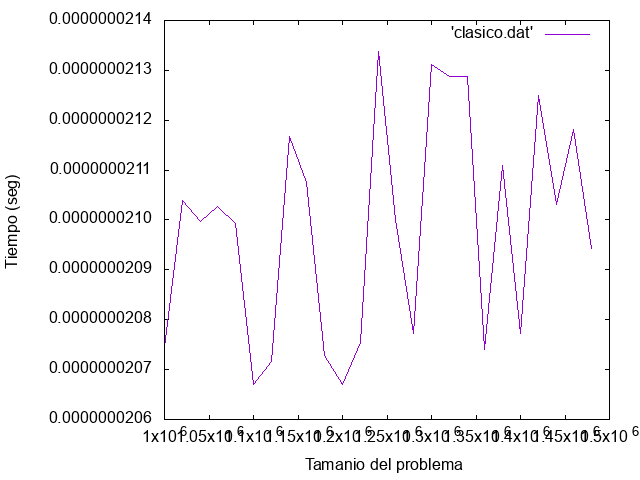
\includegraphics[scale=0.5]{clasico.png}
\end{figure}
\end{frame}

\begin{frame}[fragile]{Algoritmo Divide y Vencerás}
\begin{figure}[H]
\centering
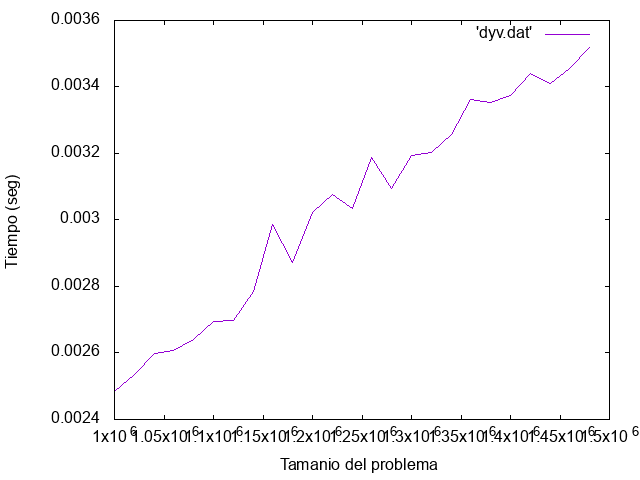
\includegraphics[scale=0.5]{dyv.png}
\end{figure}
\end{frame}

\begin{frame}[fragile]{Algoritmo Divide y Vencerás (zoom)}
\begin{figure}[H]
\centering
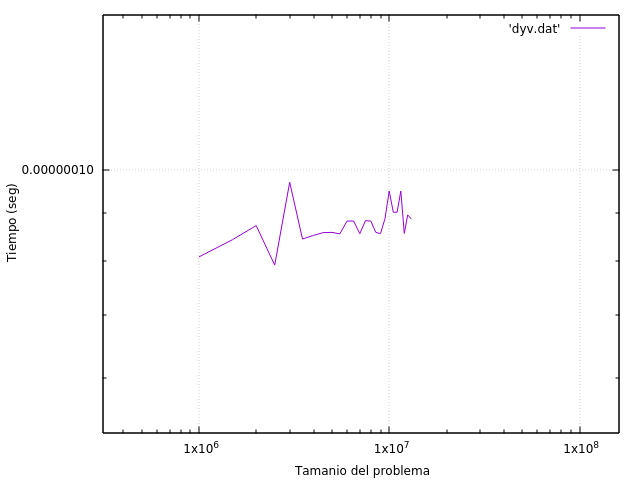
\includegraphics[scale=0.5]{dyv_zoom.png}
\end{figure}
\end{frame}


\subsubsection{Comparación entre algoritmos}
\begin{frame}[fragile]{Comparación entre ambos algoritmos}
\begin{figure}[H]
\centering
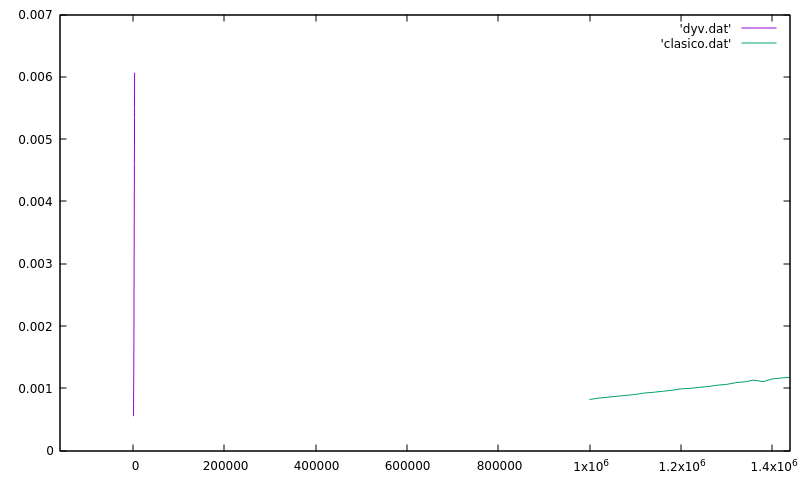
\includegraphics[scale=0.5]{empirica_ambos.png}
\end{figure}
\end{frame}


\subsection{Cálculo de la eficiencia híbrida}

\subsubsection{Errores en el cálculo de la constante oculta}

\begin{frame}[fragile]{Errores en el cálculo de la constante oculta}
\begin{table}[H]
\centering
\resizebox{\textwidth}{!}{%
\begin{tabular}{|c|c|c|c|}
\hline
\textbf{Algoritmo} & \textbf{Eficiencia teórica} & \textbf{Valor de la constante oculta} & \textbf{Error} \\
\hline
Clásico & O($n$) & 8.19304 $\cdot 10^{-10} $ &0.1441\% \\
Divide y Vencerás & O($log(n)$) & 5.61125$\cdot 10^{-9} $ & 0.9174\% \\
\hline
\end{tabular}
}
\end{table}
\end{frame}

\begin{frame}[fragile]{Algoritmo clásico}
\begin{figure}[H]
\centering
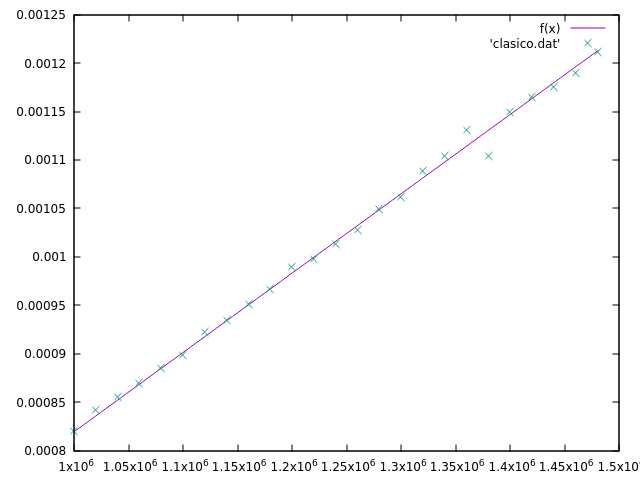
\includegraphics[scale=0.5]{hibrida_clasico.png}
\end{figure}
\end{frame}

\begin{frame}[fragile]{Algoritmo Divide y Vencerás}
\begin{figure}[H]
\centering
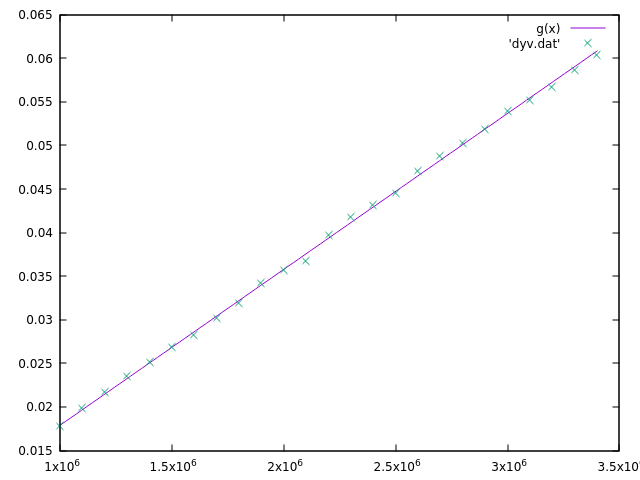
\includegraphics[scale=0.5]{hibrida_dyv.png}
\end{figure}
\end{frame}

\section{Vectores con elementos repetidos}


\begin{frame}[fragile]{Planteamiento}
¿Seguirá funcionando el algoritmo Divide y Vencerás si se repiten elementos en el vector?
\end{frame}

\begin{frame}[fragile]{Elementos repetidos (I)}
\begin{tikzpicture}[font=\ttfamily,
array/.style={matrix of nodes,nodes={draw, minimum size=7mm, fill=blue!30},column sep=-\pgflinewidth, row sep=0.5mm, nodes in empty cells,
row 1/.style={nodes={draw=none, fill=none, minimum size=5mm}}}]

\matrix[array] (array) {
0 & 1 & 2 & 3 & 4 & 5 & 6 \\
  &   &   &   &   &   &   \\};
%\node[draw, fill=gray, minimum size=4mm] at (array-2-3) (box) {};
\node at (array-2-1) {1};
\node at (array-2-2) {2};
\node at (array-2-3) {2};
\node at (array-2-4) {2};
\node at (array-2-5) {3};
\node at (array-2-6) {4};
\node at (array-2-7) {5};



\draw[<->]([yshift=-3mm]array-2-1.south west) -- node[below] {Tamaño del vector: 7} ([yshift=-3mm]array-2-7.south east);

\end{tikzpicture}
\end{frame}

\begin{frame}[fragile]{Elementos repetidos (II)}
\begin{tikzpicture}[font=\ttfamily,
array/.style={matrix of nodes,nodes={draw, minimum size=7mm, fill=blue!30},column sep=-\pgflinewidth, row sep=0.5mm, nodes in empty cells,
row 1/.style={nodes={draw=none, fill=none, minimum size=5mm}}}]

\matrix[array] (array) {
0 & 1 & \textcolor{green}{2} & 3 & 4 & 5 & 6 \\
  &   &   &   &   &   &   \\};
%\node[draw, fill=gray, minimum size=4mm] at (array-2-3) (box) {};
\node at (array-2-1) {1};
\node at (array-2-2) {2};
\node[draw, fill=green!20] at (array-2-3) {2};
\node at (array-2-4) {2};
\node at (array-2-5) {3};
\node at (array-2-6) {4};
\node at (array-2-7) {5};


\draw[<->]([yshift=-3mm]array-2-1.south west) -- node[below] {Tamaño del vector: 7} ([yshift=-3mm]array-2-7.south east);

\end{tikzpicture}
\end{frame}

\begin{frame}[fragile]{Elementos repetidos (III)}
\begin{tikzpicture}[font=\ttfamily,
array/.style={matrix of nodes,nodes={draw, minimum size=7mm, fill=blue!30},column sep=-\pgflinewidth, row sep=0.5mm, nodes in empty cells,
row 1/.style={nodes={draw=none, fill=none, minimum size=5mm}}}]

\matrix[array] (array) {
0 & 1 & \textcolor{green}{2} & 3 & 4 & 5 & 6 \\
  &   &   &   &   &   &   \\};
%\node[draw, fill=gray, minimum size=4mm] at (array-2-3) (box) {};
\node at (array-2-1) {1};
\node at (array-2-2) {2};
\node[draw, fill=green!20] at (array-2-3) {2};
\node[draw,fill=red!50] at (array-2-4) {2};
\node at (array-2-5) {3};
\node at (array-2-6) {4};
\node at (array-2-7) {5};



\draw[<->]([yshift=-3mm]array-2-1.south west) -- node[below] {Tamaño del vector: 7} ([yshift=-3mm]array-2-7.south east);

\end{tikzpicture}
\vskip 0.5 cm
Calculamos el centro del vector.\\
$mitad=\frac{ini+fin=6}{2}=$\textcolor{red}{3}

\end{frame}

\begin{frame}[fragile]{Elementos repetidos (IV)}
\begin{tikzpicture}[font=\ttfamily,
array/.style={matrix of nodes,nodes={draw, minimum size=7mm, fill=blue!30},column sep=-\pgflinewidth, row sep=0.5mm, nodes in empty cells,
row 1/.style={nodes={draw=none, fill=none, minimum size=5mm}}}]

\matrix[array] (array) {
0 & 1 & \textcolor{green}{2} & 3 & 4 & 5 & 6 \\
  &   &   &   &   &   &   \\};
%\node[draw, fill=gray, minimum size=4mm] at (array-2-3) (box) {};
\node at (array-2-1) {1};
\node at (array-2-2) {2};
\node[draw, fill=green!20] at (array-2-3) {2};
\node[draw,fill=red!50] at (array-2-4) {2};
\node at (array-2-5) {3};
\node at (array-2-6) {4};
\node at (array-2-7) {5};



\draw[<->]([yshift=-3mm]array-2-1.south west) -- node[below] {Tamaño del vector: 7} ([yshift=-3mm]array-2-7.south east);

\end{tikzpicture}
\vskip 0.5 cm
$mitad=\frac{6}{2}=$\textcolor{red}{3}
\vskip 0.5cm
¿$v[3]=3$? \textcolor{red}{NO} \\
¿$v[3]=2<3]$? \textcolor{green}{SÍ} $\rightarrow$ exploramos desde $mitad+1=4$ a $fin=6$
\end{frame}

\begin{frame}[fragile]{Elementos repetidos (V)}
\begin{tikzpicture}[font=\ttfamily,
array/.style={matrix of nodes,nodes={draw, minimum size=7mm, fill=blue!30},column sep=-\pgflinewidth, row sep=0.5mm, nodes in empty cells,
row 1/.style={nodes={draw=none, fill=none, minimum size=5mm}}}]

\matrix[array] (array) {
0 & 1 & \textcolor{green}{2} & 3 & 4 & 5 & 6 \\
  &   &   &   &   &   &   \\};
%\node[draw, fill=gray, minimum size=4mm] at (array-2-3) (box) {};
\node at (array-2-1) {1};
\node at (array-2-2) {2};
\node[draw, fill=green!20] at (array-2-3) {2};
\node[draw,fill=red!50] at (array-2-4) {2};
\node at (array-2-5) {3};
\node at (array-2-6) {4};
\node at (array-2-7) {5};


\draw[<->]([yshift=-3mm]array-2-1.south west) -- node[below] {Tamaño del vector: 7} ([yshift=-3mm]array-2-7.south east);

\end{tikzpicture}
\vskip 0.5 cm
$mitad=\frac{6}{2}=$\textcolor{red}{3} 

\begin{tikzpicture}[font=\ttfamily,
array/.style={matrix of nodes,nodes={draw, minimum size=7mm, fill=blue!30},column sep=-\pgflinewidth, row sep=0.5mm, nodes in empty cells,
row 1/.style={nodes={draw=none, fill=none, minimum size=5mm}}}]

\matrix[array] (array) {
4 & 5 & 6 \\
 &   &   \\};
%\node[draw, fill=gray, minimum size=4mm] at (array-2-3) (box) {};

\node at (array-2-1) {3};
\node at (array-2-2) {4};
\node at (array-2-3) {5};

\draw[<->]([yshift=-3mm]array-2-1.south west) -- node[below] {Tamaño del vector: 3} ([yshift=-3mm]array-2-3.south east);

\end{tikzpicture}

Al repetirse elementos, destruimos uno de los axiomas principales de la estrategia Divide y Vencerás $\rightarrow$ El algoritmo \textcolor{red}{no} es válido.
\end{frame}

\begin{frame}[fragile]{Sin embargo...}
Hay un caso en el que puede funcionar: si en alguna iteración $v[mitad]=mitad$.\\
\begin{tikzpicture}[font=\ttfamily,
array/.style={matrix of nodes,nodes={draw, minimum size=7mm, fill=blue!30},column sep=-\pgflinewidth, row sep=0.5mm, nodes in empty cells,
row 1/.style={nodes={draw=none, fill=none, minimum size=5mm}}}]

\matrix[array] (array) {
0 & 1 & \textcolor{green}{2} & 3 & 4 & \textcolor{green}{5} & 6 \\
  &   &   &   &   &   &   \\};
%\node[draw, fill=gray, minimum size=4mm] at (array-2-3) (box) {};
\node at (array-2-1) {1};
\node at (array-2-2) {2};
\node[draw, fill=green!20] at (array-2-3) {2};
\node[draw,fill=red!50] at (array-2-4) {2};
\node at (array-2-5) {3};
\node[draw, fill=green!20] at (array-2-6) {5};
\node at (array-2-7) {5};


\draw[<->]([yshift=-3mm]array-2-1.south west) -- node[below] {Tamaño del vector: 7} ([yshift=-3mm]array-2-7.south east);

\end{tikzpicture}

\vskip 0.5cm

\begin{tikzpicture}[font=\ttfamily,
array/.style={matrix of nodes,nodes={draw, minimum size=7mm, fill=blue!30},column sep=-\pgflinewidth, row sep=0.5mm, nodes in empty cells,
row 1/.style={nodes={draw=none, fill=none, minimum size=5mm}}}]

\matrix[array] (array) {
4 &  \textcolor{green}{5} & 6 \\
 &   &   \\};
%\node[draw, fill=gray, minimum size=4mm] at (array-2-3) (box) {};

\node at (array-2-1) {3};
\node[draw, fill=green!20] at (array-2-2) {5};
\node at (array-2-3) {5};

\draw[<->]([yshift=-3mm]array-2-1.south west) -- node[below] {Tamaño del vector: 3} ([yshift=-3mm]array-2-3.south east);

\end{tikzpicture}

\end{frame}

\section*{Fin de la presentación}

\begin{frame}{Fin}
\begin{center}
\huge{Fin de la presentación}
\end{center}
\end{frame}


\end{document}


